\section{凸优化}
\subsection{凸分析基础}
\begin{definition}[Lipschitz连续]
    \[
        \lvert f(\boldsymbol{x})-f(\boldsymbol{y})\rvert\leqslant L\lVert\boldsymbol{x}-\boldsymbol{y}\rVert,\quad\forall\boldsymbol{x},\boldsymbol{y}\in\mathbb{R}^n   
    \]
\end{definition}
\begin{definition}[局部Lipschitz连续]
    \[
        |f(\boldsymbol{x})-f(\boldsymbol{y})|\leqslant L_{\boldsymbol{x}_0}\|\boldsymbol{x}-\boldsymbol{y}\|,\quad\forall\boldsymbol{x},\boldsymbol{y}\in N(\boldsymbol{x}_0,\delta)
    \]
\end{definition}
\begin{definition}[正常函数]
    $f:\mathbb{R}^n\to\mathbb{R}$满足$f(x)>-\infty,\quad\forall x\in\mathbb{R}^n$且存在$\bar{\boldsymbol{x}}\in\mathbb{R}^n$使得$f(\boldsymbol{\bar{x}})<\infty$。\colorbox{red!50}{($f(\boldsymbol{x})$有下确界,且不恒取无穷大)}
\end{definition}
\begin{theorem}
    正常凸函数在其定义域内部局部Lipschitz连续.
\end{theorem}
\begin{theorem}
    设$f:\mathbb{R}^n\to \mathbb{R}$为正常凸函数,则对任意$\boldsymbol{x,d}\in\mathbb{R}^n$,
    \[
        \dfrac{f(\boldsymbol{x}+t\boldsymbol{d})-f(\boldsymbol{x})}{t}\colorbox{cyan!50}{关于$t$单调递增}
    \]
    或者说:对凸函数, 沿任一方向, 若函数值增长则逐渐加快,否则逐渐变慢.方向导数$\lim\limits_{t\to 0+}\dfrac{f(\boldsymbol{x}+t\boldsymbol{d})-f(\boldsymbol{x})}t$存在
    \begin{figure}[htbp]
        \centering
        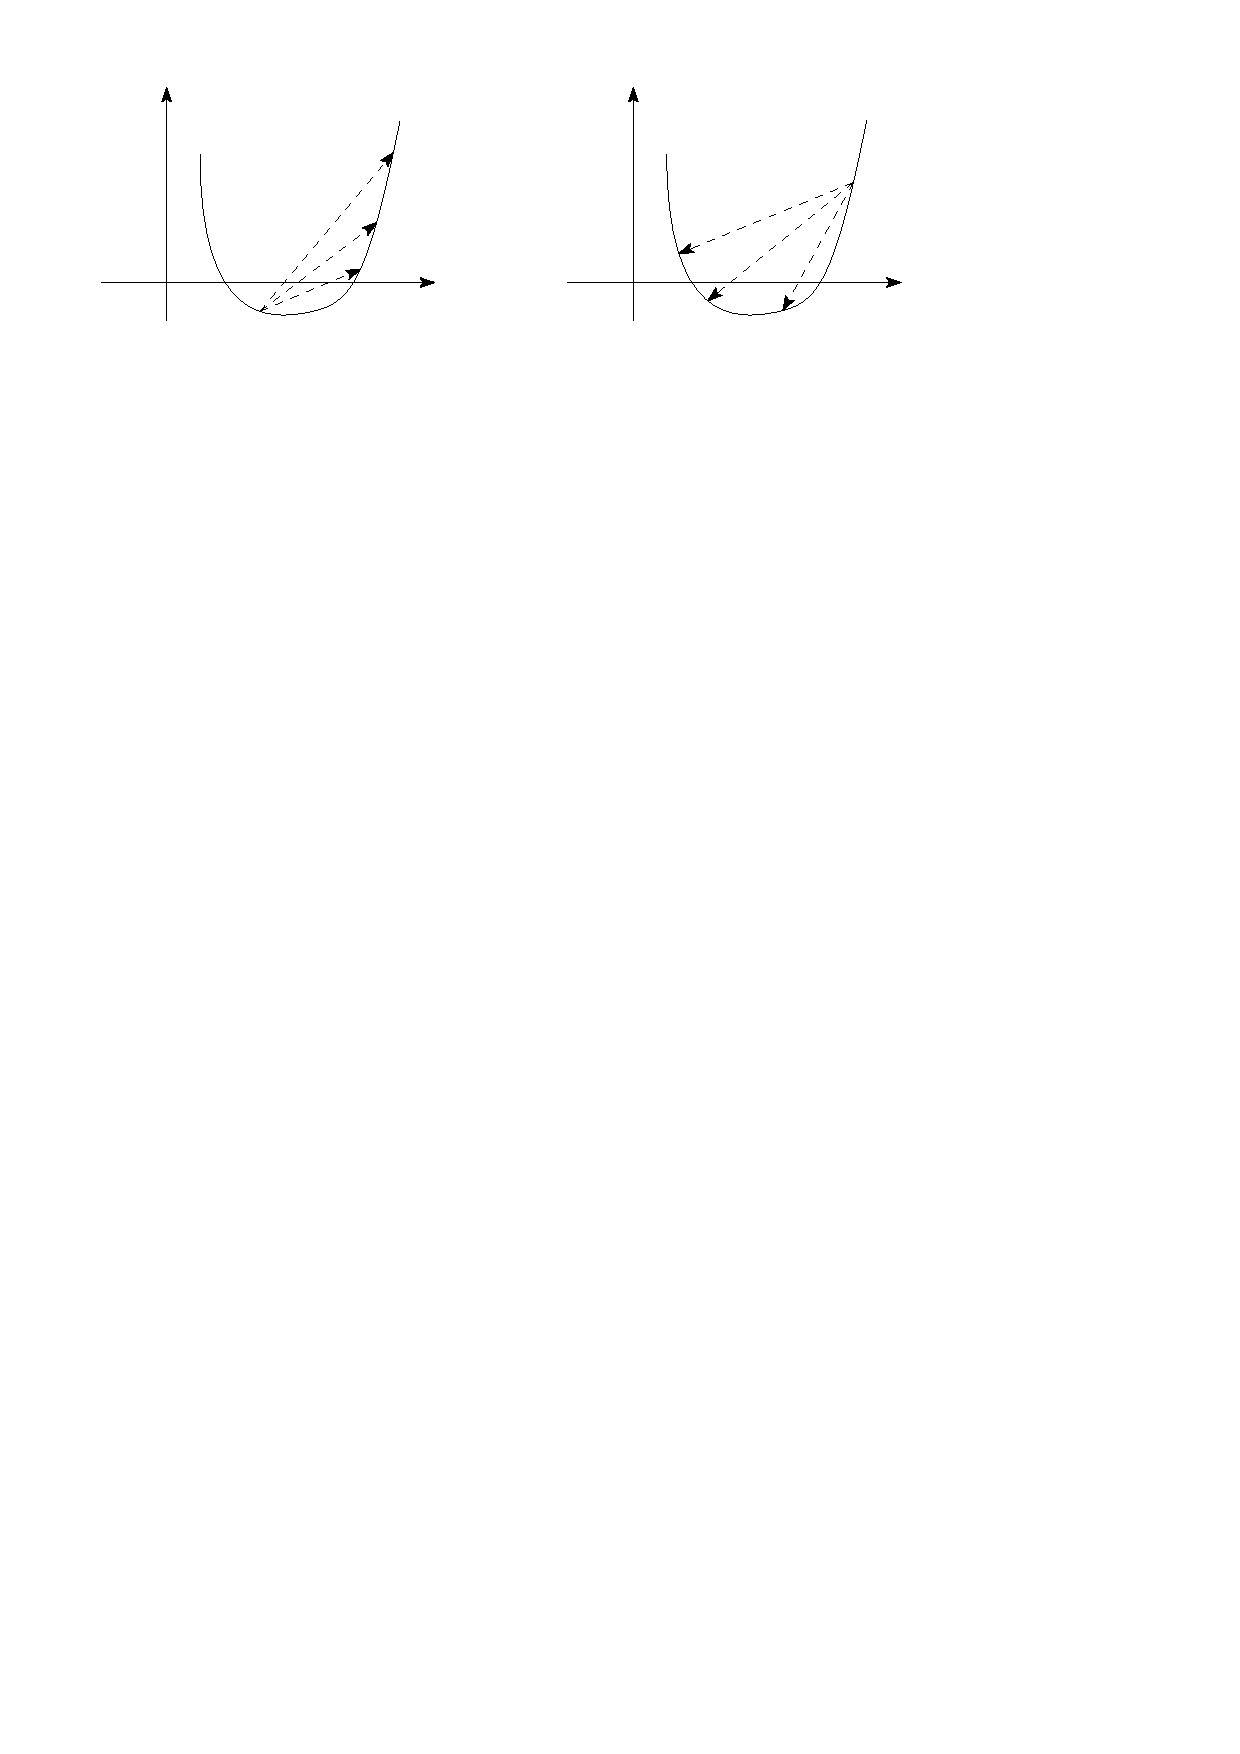
\includegraphics[scale = 0.8]{image/凸函数定理.pdf}
    \end{figure}
\end{theorem}
\begin{definition}[次梯度]
    非光滑图凸函数:存在$\boldsymbol{\xi}\in\mathbb{R}^n$使得
    \[
        f(\boldsymbol{y})\geqslant f(\boldsymbol{x})+\langle\boldsymbol{\xi},\boldsymbol{y}-\boldsymbol{x}\rangle,\quad\forall\boldsymbol{y}\in\mathbb{R}^n,
    \]
    $\boldsymbol{\xi}$称为凸函数$f(\boldsymbol{x})$在$x$点的次梯度。
\end{definition}
\begin{definition}[次微分]
    满足
    \[
        \partial f(\boldsymbol{x})=\{\boldsymbol{\xi}\in\mathbb{R}^n\mid f(\boldsymbol{y})\geqslant f(\boldsymbol{x})+\langle\boldsymbol{\xi},\boldsymbol{y}-\boldsymbol{x}\rangle,\forall\boldsymbol{y}\in\mathbb{R}^n\}.
    \]
    称
    \[
        h(\boldsymbol{y})\triangleq f(\boldsymbol{x})+\langle\boldsymbol{\xi},\boldsymbol{y}-\boldsymbol{x}\rangle 
    \]
    为函数$f(\boldsymbol{x})$在$\boldsymbol{x}$点的支撑超平面。
    \begin{figure}[htbp]
        \centering
        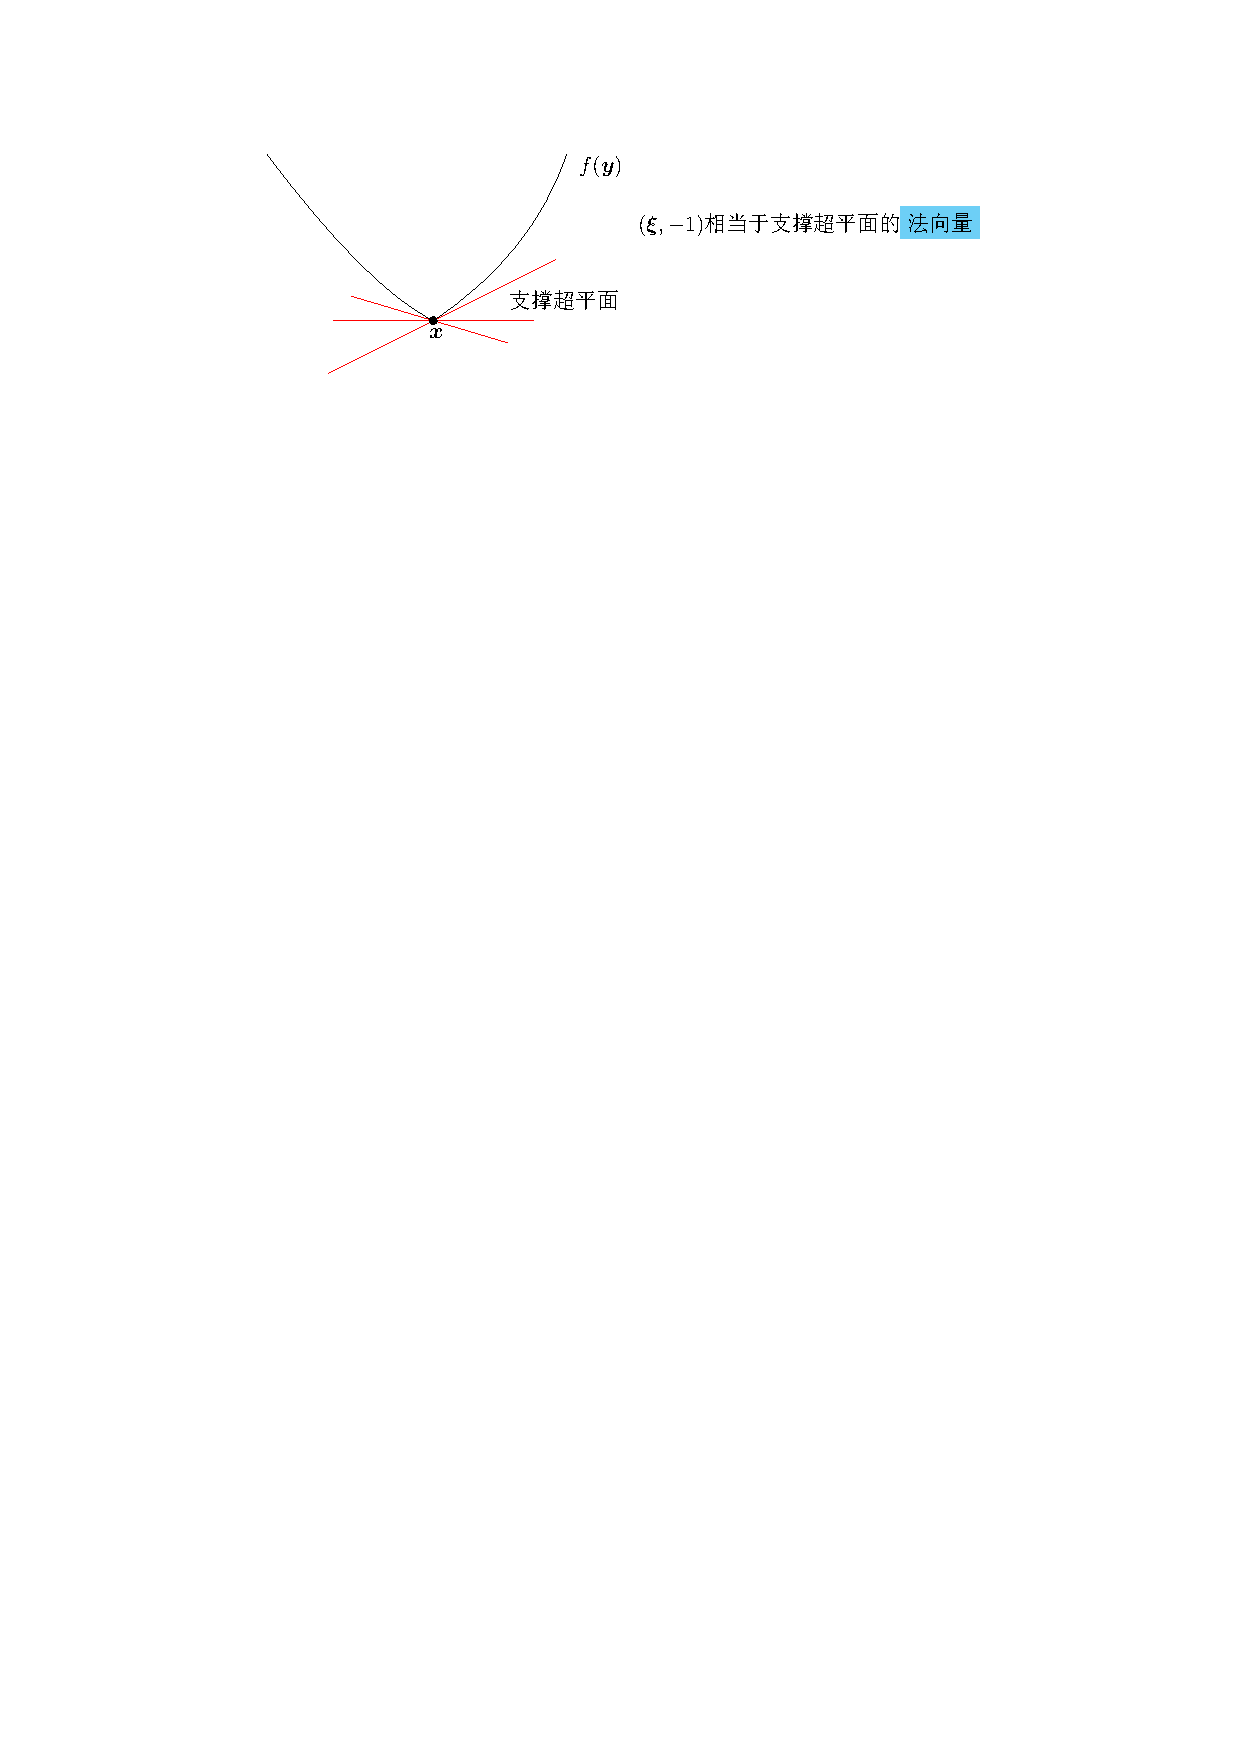
\includegraphics{image/支撑超平面.pdf}
    \end{figure}
\end{definition}
\begin{note}
    次梯度可能存在,可能不存在,也可能存在不唯一。
\end{note}
\begin{example}
    凸函数$f(x)=\begin{cases}-\sqrt{x},&x\geqslant0\\[2ex]\infty,&\text{else}\end{cases}$在零点没有次微分
    \begin{figure}[htbp]
        \centering
        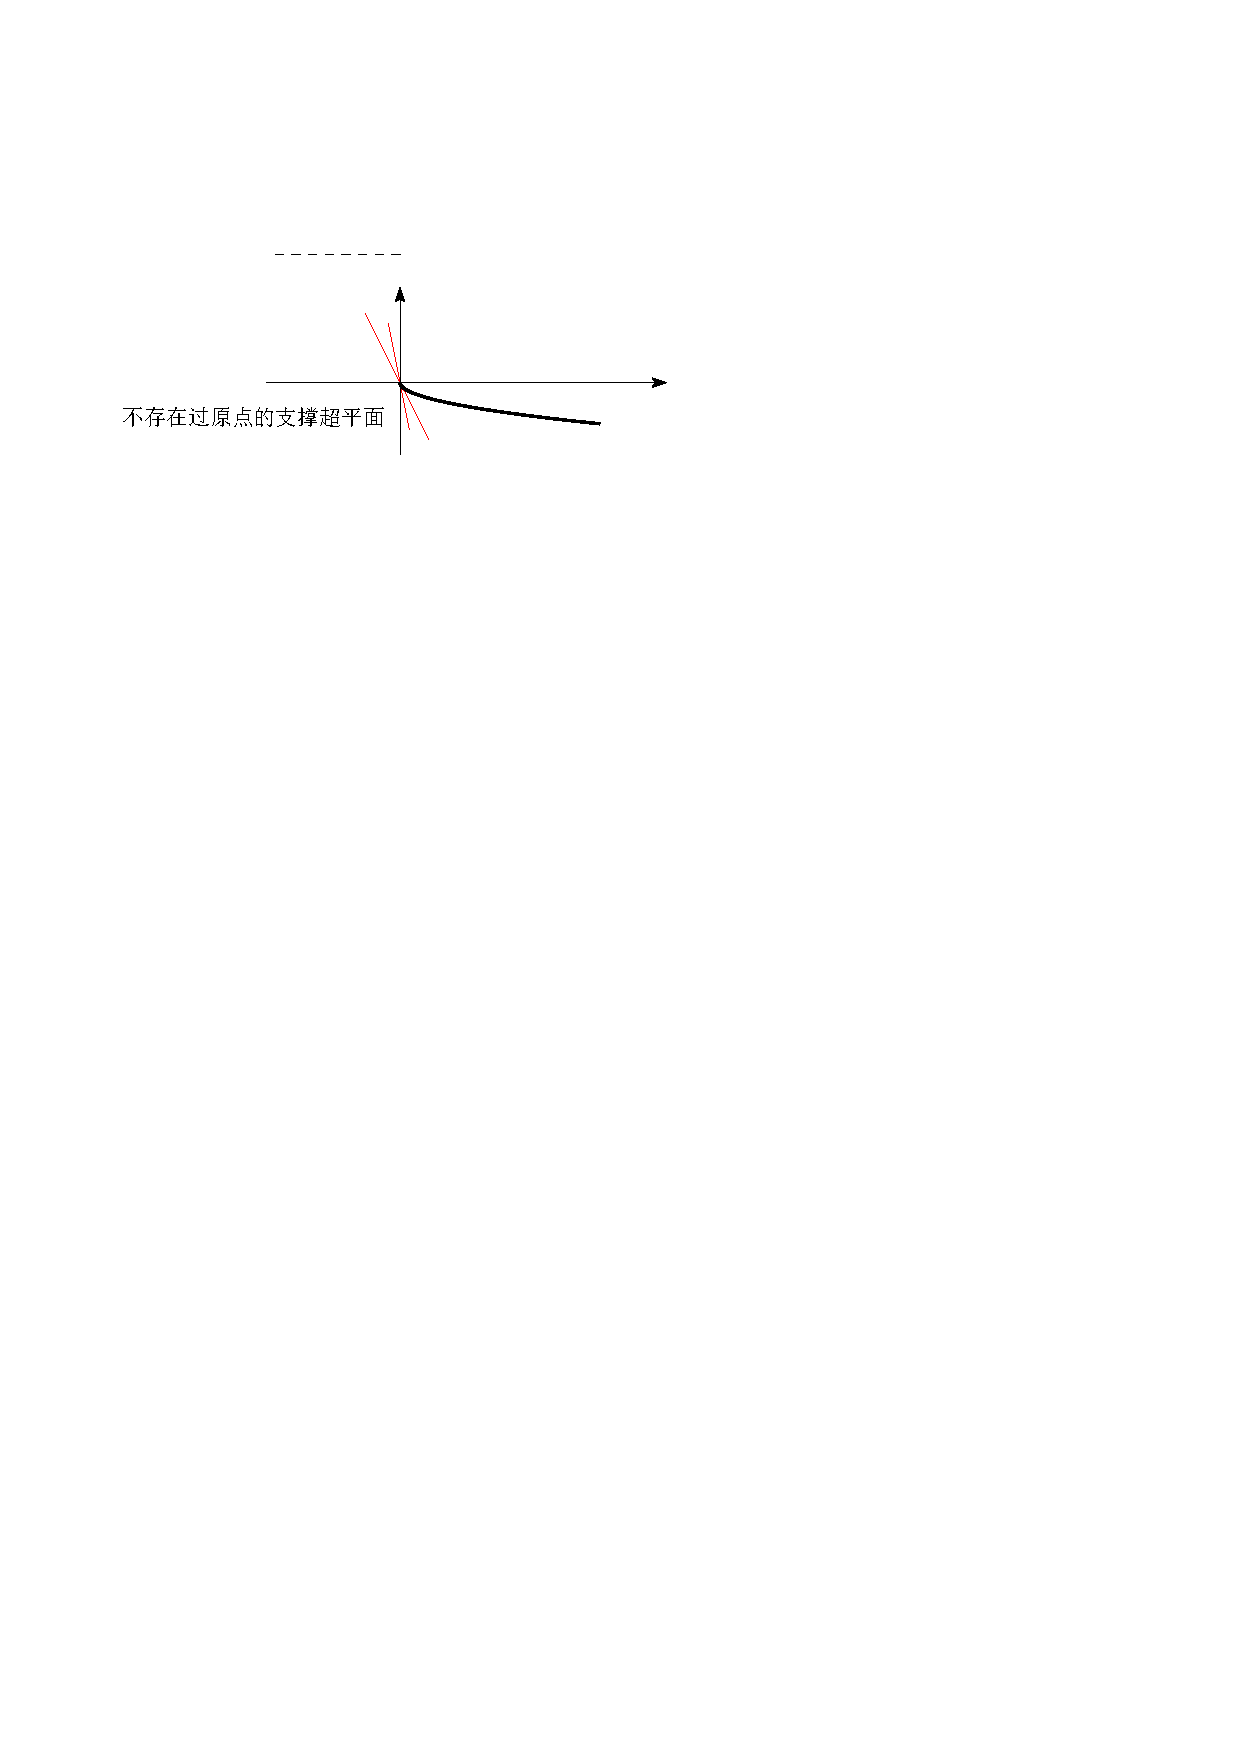
\includegraphics{image/支撑超平面example.pdf}
    \end{figure}
\end{example}
\begin{theorem}
    对凸函数$f:\mathbb{R}^n\to\mathbb{R}$,有
    \[
        \boldsymbol{\xi}\in\partial f(\boldsymbol{x})\Longleftrightarrow f'(\boldsymbol{x};\boldsymbol{d})\geqslant\boldsymbol{\xi}^\mathrm{T}\boldsymbol{d},\quad\forall \boldsymbol{d}\in\mathbb{R}^n.
    \]
\end{theorem}
\begin{theorem}
    $\boldsymbol{x}^*\in\mathbb{R}^n$为凸函数$f:\mathbb{R}^n\to\mathbb{R}$的最优值点当且仅当$\mathbf{0}\in\partial f(\boldsymbol{x})^*$
\end{theorem}
\begin{proof}
    \[
        \begin{array}{l}
            \mathbf{0}\in\partial f(\boldsymbol{x}^*)\\
            f(\boldsymbol{x})\geqslant f(\boldsymbol{x}^*)+\langle\boldsymbol{0},\boldsymbol{x}-\boldsymbol{x}^*\rangle,\quad\forall\boldsymbol{x}\in\mathbb{R}^n\\
            f(\boldsymbol{x})\geqslant f(\boldsymbol{x}^*),\quad\forall\boldsymbol{x}\in\mathbb{R}^n
        \end{array}
    \]
    证毕!
\end{proof}
\begin{note}
    次梯度是凸函数梯度的推广. 如果凸函数连续可微,则\colorbox{cyan!50}{梯度=次梯度}.
\end{note}
\begin{theorem}
    若凸函数$f:\mathbb{R}^n\to\mathbb{R}$在$\boldsymbol{x}$点可微,则
    \[
        \partial f(\boldsymbol{x})=\{\nabla f(\boldsymbol{x})\}
    \]
\end{theorem}
\begin{theorem}
    凸函数$f:\mathbb{R}^n\to\mathbb{R}$和其定义域内任一内点$\boldsymbol{x}$,$\partial f(x)$非空有界.
\end{theorem}
\begin{note}
    \colorbox{cyan!50}{凸函数一定次可微!可行域边界点除外。}
\end{note}
\begin{theorem}
    若$f:\mathbb{R}^n\to\mathbb{R}$在其定义域内部次可微, 则它为凸函数。
\end{theorem}
\begin{note}
    次梯度的推广:
    \begin{itemize}
        \item 非凸Lipschitz连续
        \[
            |f(\boldsymbol{x})-f(\boldsymbol{y})|\leqslant L\|\boldsymbol{x}-\boldsymbol{y}\|,\quad\forall\boldsymbol{x},\boldsymbol{y}\in\mathbb{R}^n
        \]
        \item 非凸局部Lipschitz连续
        \[
            |f(\boldsymbol{x})-f(\boldsymbol{y})|\leqslant L_{\boldsymbol{x}_0}\|\boldsymbol{x}-\boldsymbol{y}\|,\quad\forall\boldsymbol{x},\boldsymbol{y}\in N(\boldsymbol{x}_0,\delta)
        \]
    \end{itemize}
\end{note}
\subsubsection{临近点算子}
\begin{definition}[临近点算子]
    对函数$f:\mathbb{R}^n\to\mathbb{R}$,定义其在$\boldsymbol{x}\in\mathbb{R}^n$点的临近点算子
    \[
        \operatorname{prox}_f(\boldsymbol{x})=\arg\min_{\boldsymbol{y}\in\mathbb{R}^n}\Big\{f(\boldsymbol{y})+\frac{1}{2}\|\boldsymbol{y}-\boldsymbol{x}\|^2\Big\}
    \]
\end{definition}
\begin{note}
    临近点算子使子问题的性能得到加强, 如非凸函数变为凸函数,凸函数变为强凸函数, 便于在当前迭代点临近找到比该点更好的点.
\end{note}
\begin{definition}[临近点算子的扩展]
    \[
        \begin{aligned}
            \mathrm{prox}_{\frac{1}{L}f}(\boldsymbol{x})& =\underset{\boldsymbol{y}\in\mathbb{R}^{n}}{\arg\min}\Big\{f(\boldsymbol{y})+\frac{L}{2}\|\boldsymbol{y}-\boldsymbol{x}\|^{2}\Big\}  \\
            &=\underset{\boldsymbol{y}\in\mathbb{R}^{n}}{\arg\min}\Big\{\frac{1}{L}f\big(\boldsymbol{y}\big)+\frac{1}{2}\big\Vert\boldsymbol{y}-\boldsymbol{x}\big\Vert^{2}\Big\}
        \end{aligned}
    \]
    对于$f(\boldsymbol{x})+g(\boldsymbol{x})$,$f:\mathbb{R}^n\to\mathbb{R}$连续可微,$g:\mathbb{R}^n\to\mathbb{R}$连续
    \[
        \begin{array}{l}
            \arg\min\limits_{\boldsymbol{x}\in\mathbb{R}^{n}}\Big\{f(\boldsymbol{x}_{0})+\textcolor{red!50}{\underline{\nabla f(\boldsymbol{x}_{0})^{\mathrm{T}}(\boldsymbol{x}-\boldsymbol{x}_{0})+\dfrac{L}{2}\|\boldsymbol{x}-\boldsymbol{x}_{0}\|^{2}}}+g(\boldsymbol{x})\Big\}\\
            =\arg\operatorname*{min}\limits_{\boldsymbol{x}\in\mathbb{R}^{n}}\Big\{\dfrac{1}{L}g(\boldsymbol{x})+\textcolor{red!50}{\underline{\dfrac{1}{2}\|\boldsymbol{x}-\Big(\boldsymbol{x}_{0}-\dfrac{1}{L}\nabla f(\boldsymbol{x}_{0})\Big)\|^{2}}}\Big\}\\
            \stackrel{\triangle}{=}\mathrm{prox}_{\frac{1}{L}g}\bigl(\boldsymbol{x}_{0}-\dfrac{1}{L}\nabla f(\boldsymbol{x}_{0})\bigr)
        \end{array}
    \]
\end{definition}
\begin{example}
    求$f_2(x)=\begin{cases}0,&x\neq0\\[2ex]-\lambda,&x=0\end{cases}$的临近点算子$(\lambda>0)$。\Stars{5}{}

    \[
        \begin{aligned}
            \mathrm{prox}_{f_{2}}(x)& =\arg\min_{y\in\mathbb{R}}\left\{f_{2}(y)+\frac{1}{2}(y-x)^{2}\right\}  \\
            &=\arg\min_{y\in\mathbb{R}}\left\{\min_{y=0}\left\{-\lambda+\frac{x^{2}}{2}\right\},\min_{y\neq0}\left\{\frac{1}{2}(y-x)^{2}\right\}\right\} \\
            &=\arg\min_{y\in\mathbb{R}}\left\{-\lambda+\frac{x^{2}}{2},0\right\} \\
            &\left.=\left\{\begin{array}{ll}\{0\},&|x|<\sqrt{2\lambda}\\[2ex]\{x\},&|x|>\sqrt{2\lambda}\\[2ex]\{0,x\},&|x|=\sqrt{2\lambda}\end{array}\right.\right.
        \end{aligned}
    \]    
\end{example}
\begin{example}
    求$f_3(x)=\begin{cases}0,&x\neq0\\[2ex]\lambda,&x=0\end{cases}$的临近点算子$(\lambda>0)$。\Stars{5}{}

    解:
    \[
        \mathrm{prox}_{f_3}(x)=
            \left\{
                \begin{array}{cc}
                    \{x\}, & x\neq0\\
                    \emptyset, & x=0
                \end{array}
            \right.
    \]
\end{example}
\begin{definition}[下半连续]
    \[
        \lim_{\boldsymbol{x}\to\boldsymbol{x}_0}\inf f(\boldsymbol{x})\geqslant f(\boldsymbol{x}_0)
    \]
    \begin{figure}[htbp]
        \centering
        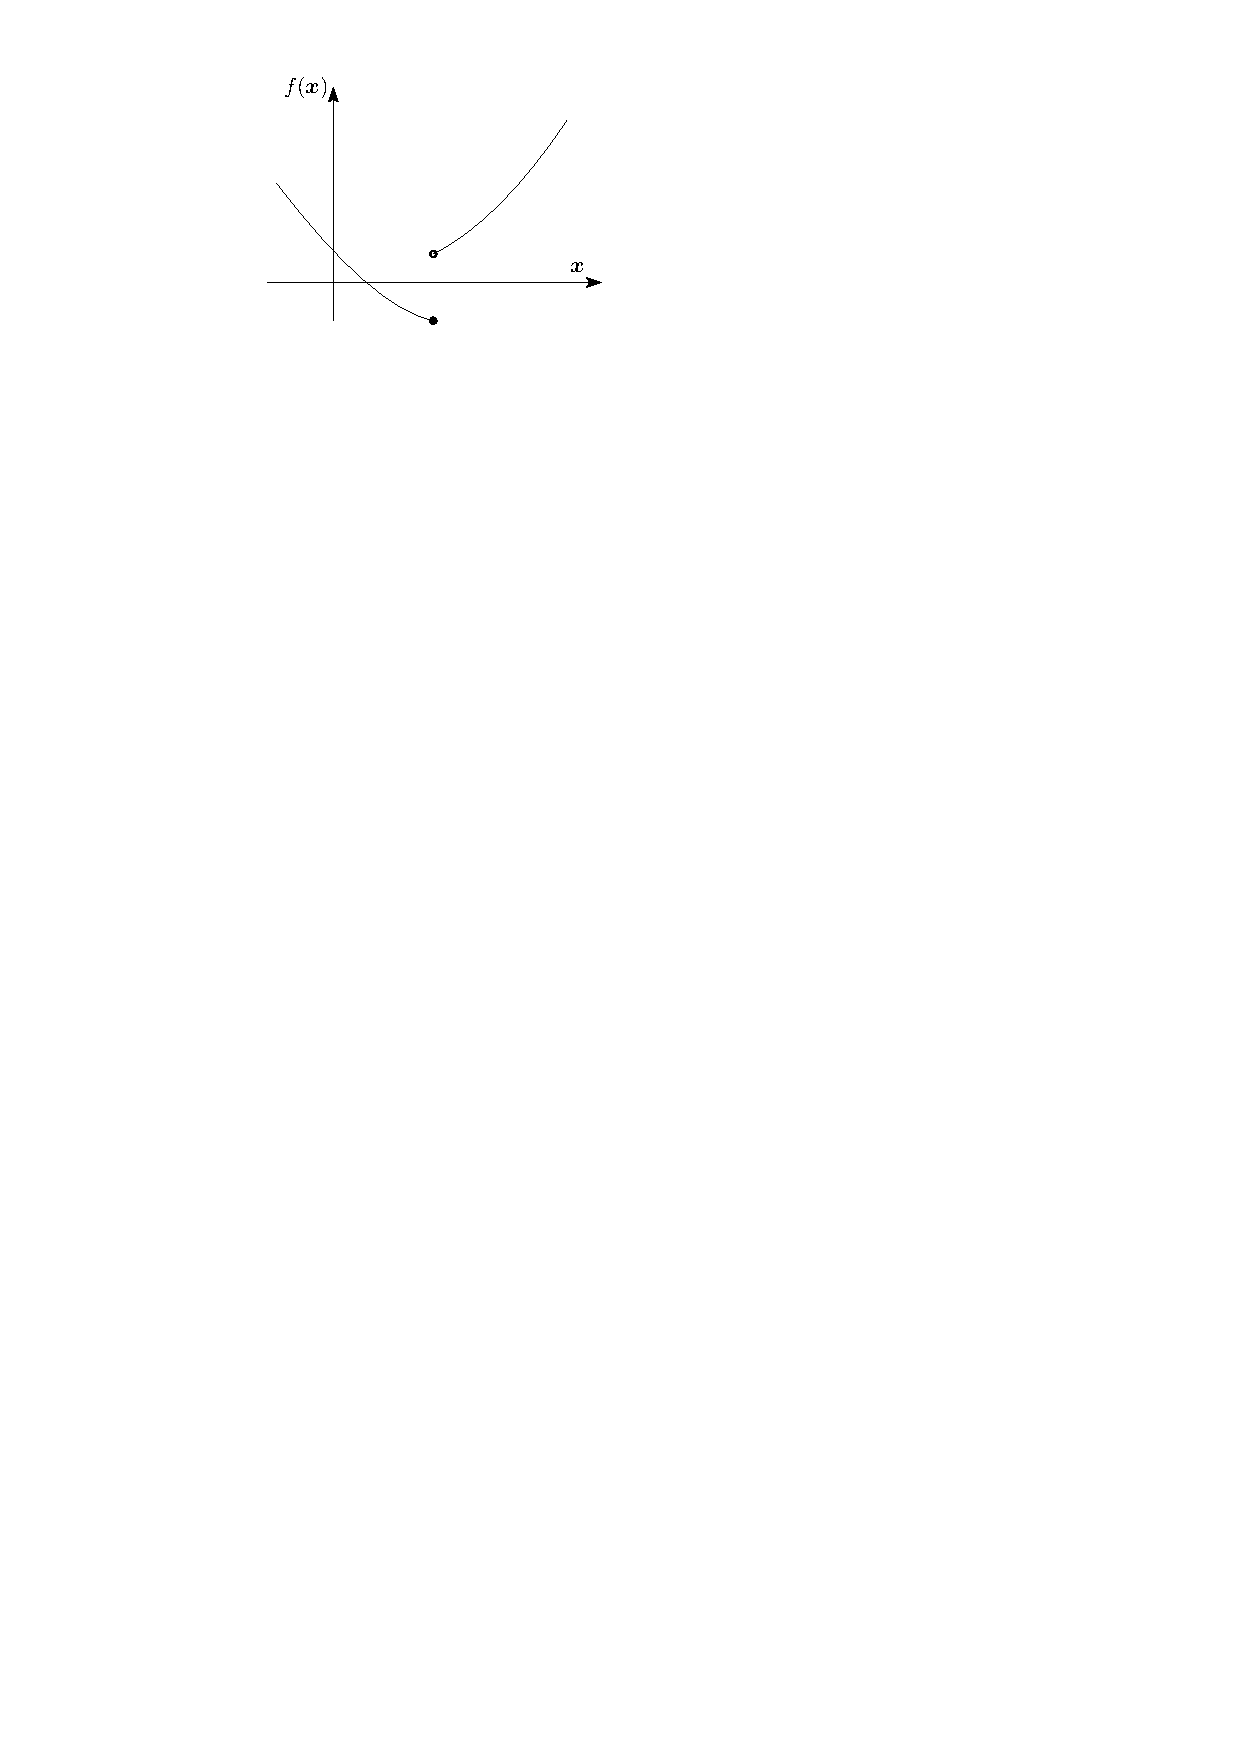
\includegraphics{image/下半连续.pdf}
    \end{figure}
\end{definition}
\begin{theorem}
    对下半连续的凸函数$f:\mathbb{R}^n\to\mathbb{R}$其临近点算子$\mathrm{prox}_{f}(\cdot)$为单一映射。
\end{theorem}
\begin{theorem}
    设凸函数$f:\mathbb{R}^n\to\mathbb{R}$下半连续.则对任意的$\boldsymbol{x},\boldsymbol{y}\in \mathbb{R}^{n}$ 
    \[
        \boldsymbol{y}=\mathrm{prox}_f(\boldsymbol{x})
    \]         
    \[
        \boldsymbol{x}-\boldsymbol{y}\in\partial f(\boldsymbol{y})
    \]
    \[
        \langle \boldsymbol{x}-\boldsymbol{y},\boldsymbol{z}-\boldsymbol{y}\rangle\leqslant f(\boldsymbol{z})-f(\boldsymbol{y}),\forall \boldsymbol{z}\in \mathbb{R}^{n}
    \]
\end{theorem}
\begin{proof}
    由临近点算子的定义,对任意的$\boldsymbol{x},\boldsymbol{y}\in \mathbb{R}^n$
    \[
        \boldsymbol{y}=\mathrm{prox}_{f}(\boldsymbol{x})\Longleftrightarrow \boldsymbol{y}=\arg\min_{\boldsymbol{z}\in\mathbb{R}^{n}}\{f(\boldsymbol{z})+\frac{1}{2}\|\boldsymbol{z}-\boldsymbol{x}\|^{2}\}.
    \]
    后面等价于$\boldsymbol{0}\in\partial f(\boldsymbol{y})+\boldsymbol{y}-\boldsymbol{x}.$
    由次梯度的定义$\boldsymbol{x}-\boldsymbol{y}\in\partial f(\boldsymbol{y})$等价于,
    \[
        \langle \boldsymbol{x}-\boldsymbol{y},\boldsymbol{z}-\boldsymbol{y}\rangle\leqslant f(\boldsymbol{z})-f(\boldsymbol{y}),\forall \boldsymbol{z}\in \mathbb{R}^{n}
    \]
    证毕!
\end{proof}
\begin{theorem}
   设$f$为下半连续的凸函数. 则对任意$\boldsymbol{x},\boldsymbol{y}\in \mathbb{R}^n$
   \[
        \langle\boldsymbol{x}-\boldsymbol{y},\mathrm{prox}_f(\boldsymbol{x})-\mathrm{prox}_f(\boldsymbol{y})\rangle\geqslant\|\mathrm{prox}_f(\boldsymbol{x})-\mathrm{prox}_f(\boldsymbol{y})\|^2
   \]
   \[
        \|\mathrm{prox}_f(\boldsymbol{x})-\mathrm{prox}_f(\boldsymbol{y})\|\leqslant\|\boldsymbol{x}-\boldsymbol{y}\|.
   \]
\end{theorem}
\subsubsection{和式优化最优性条件}
为充分利用函数的解析性质,将目标函数中的项根据其解析性质分开,可得如下和式优化问题
\[
    \min_{\boldsymbol{x}\in\mathbb{R}^n}f(\boldsymbol{x})+g(\boldsymbol{x})
\]
用梯度和次梯度建立优化问题的最优性条件
\begin{theorem}
    $\boldsymbol{x}^*\in\mathbb{R}^n$为优化问题$\operatorname*{min}_{\boldsymbol{x}\in\mathbb{R}^n}f(\boldsymbol{x})+g(\boldsymbol{x})$的最优解,则$-\nabla f(\boldsymbol{x}^*)\in\partial g(\boldsymbol{x}^*)$
\end{theorem}
% \begin{proof}
%     任取$\boldsymbol{x}\mathbb{}$
% \end{proof}
\subsection{线性化临近点方法}
用梯度和函数值建立优化问题的最优性条件
\[
    \min f(\boldsymbol{x})+g(\boldsymbol{x})
\]
其中$\Omega\subset\mathbb{R}^n$,$f:\mathbb{R}^n\to\mathbb{R}$连续可微的凸函数,$g:\mathbb R^n\to\mathbb R$凸函数
\begin{theorem}
    为上述优化问题的最优解当且仅当
    \[
        g(\boldsymbol{x})-g(\boldsymbol{x}^*)+\nabla f(\boldsymbol{x}^*)^\mathrm{T}(\boldsymbol{x}-\boldsymbol{x}^*)\geqslant 0,\quad\forall\boldsymbol{x}\in\mathbb{R}^n
    \]
\end{theorem}
\begin{note}
    临近点算法
    \[
        \boldsymbol{x}_{k+1}=\arg\min_{\boldsymbol{x}\epsilon\mathbb{R}^{n}}\left\{f(\boldsymbol{x})+\frac{L}{2}\|\boldsymbol{x}-\boldsymbol{x}_{k}\|^{2}\right\}
    \]
\end{note}
\begin{note}
    算法收敛性
    \[
        \boldsymbol{x}_{k+1}=\arg\min_{\boldsymbol{x}\in\mathbb{R}^n}\left\{f(\boldsymbol{x})+\frac{L}{2}\|\boldsymbol{x}-\boldsymbol{x}_k\|^2\right\}
    \]
    由
    \begin{figure}[H]
        \centering
        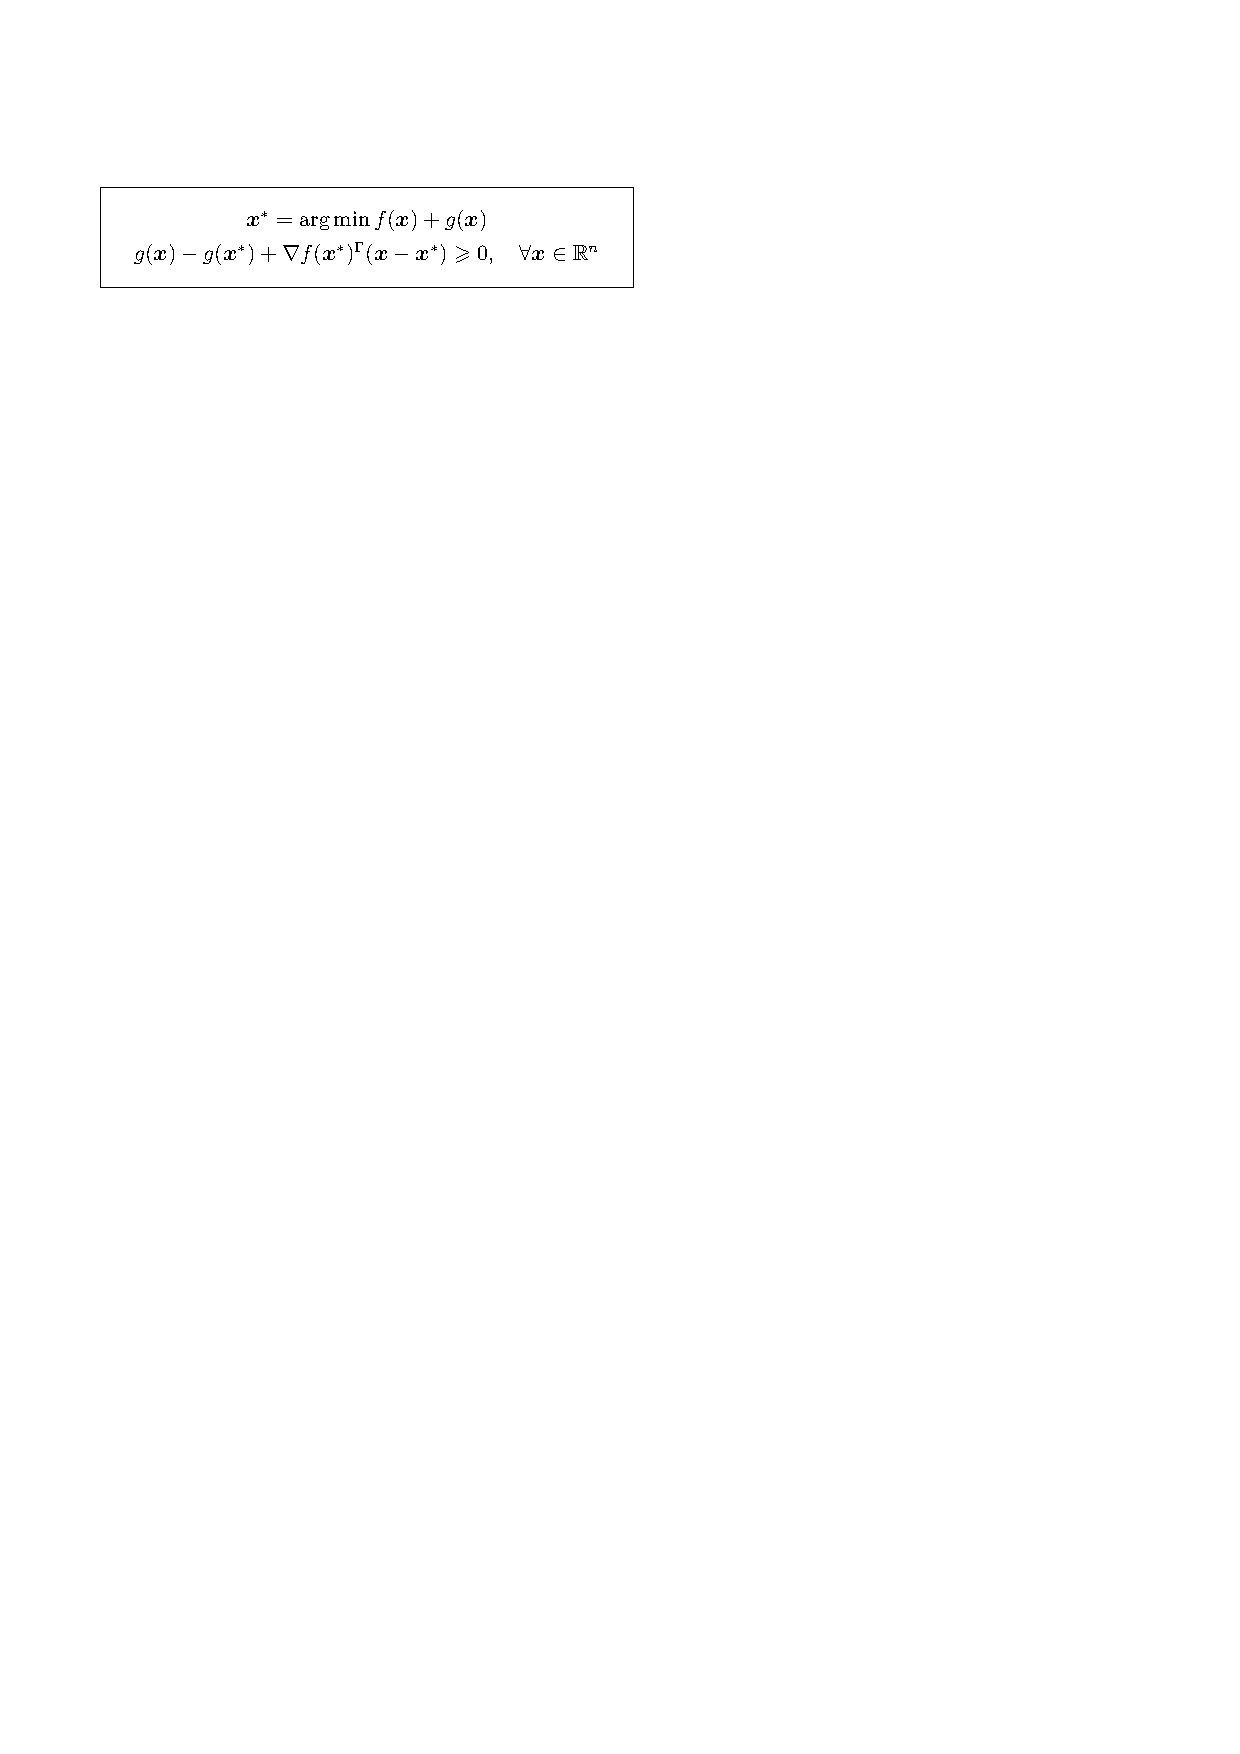
\includegraphics{image/临近点算子收敛性.pdf}
    \end{figure}
    得
    \[
        f(\boldsymbol{x})-f(\boldsymbol{x}_{k+1})+L(\boldsymbol{x}_{k+1}-\boldsymbol{x}_k)^\mathrm{T}(\boldsymbol{x}-\boldsymbol{x}_{k+1})\geqslant0,\quad\forall\boldsymbol{x}\in\mathbb{R}^n
    \]
    令$\boldsymbol{x} = \boldsymbol{x}_{k}$
    \[
        f(\boldsymbol{x}_k)-f(\boldsymbol{x}_{k+1})\geqslant L\|\boldsymbol{x}_k-\boldsymbol{x}_{k+1}\|^2.
    \]
    \[
        f(\boldsymbol{x}_0)-\lim_{k\to\infty}f(\boldsymbol{x}_k)\geqslant L\sum_{k=0}^\infty\|\boldsymbol{x}_k-\boldsymbol{x}_{k+1}\|^2\longrightarrow\lim_{k\to\infty}\|\boldsymbol{x}_k-\boldsymbol{x}_{k+1}\|=0.
    \]
    算法产生的函数值序列$\left\{ f(\boldsymbol{x}) \right\}$单调不增.如果目标函数$f(\boldsymbol{x})$在$\mathbb{R}^n$上有下界, 则数列$\left\{ f(\boldsymbol{x}) \right\}$收敛. 
\end{note}
\begin{theorem}
    $f:\mathbb{R}^n\to\mathbb{R}$下半连续的凸函数,有下界;临近点算法$\boldsymbol{x}_{k+1}=\mathrm{prox}_{\frac1Lf}(\boldsymbol{x}_k)$产生迭代点列的任一聚点为凸优化问题$\min\limits_{\boldsymbol{x}\in\mathbb{R}^{n}}f(\boldsymbol{x})$的最优值点.

\end{theorem}
\subsection{交替极小化方法}
\[
    \min_{\boldsymbol{x}_1\in\mathbb{R}^{n_1},\boldsymbol{x}_2\in\mathbb{R}^{n_2},\cdots,\boldsymbol{x}_s\in\mathbb{R}^{n_s}}\Psi(\boldsymbol{x}_1,\boldsymbol{x}_2,\cdots,\boldsymbol{x}_s)
\]
以循环方式交替对$s$个块变量求最小。
对迭代点$\boldsymbol{x}^k=(\boldsymbol{x}_1^k,\boldsymbol{x}_2^k,\cdotp\cdotp\cdotp,\boldsymbol{x}_s^k), $分别基于块变量依次对$\boldsymbol{x}_1,\boldsymbol{x}_2,\cdots,\boldsymbol{x}_s$求极小, 得到新的迭代点
\[
    \begin{aligned}
        &\boldsymbol{x}^{k,1}=(\boldsymbol{x}_{1}^{k+1},\boldsymbol{x}_{2}^{k},\cdots,\boldsymbol{x}_{s}^{k}),\\
        &\boldsymbol{x}^{k,2}=(\boldsymbol{x}_{1}^{k+1},\boldsymbol{x}_{2}^{k+1},\boldsymbol{x}_{3}^{k},\cdots,\boldsymbol{x}_{s}^{k}),\\
        &\boldsymbol{x}^{k,i}=(\boldsymbol{x}_{1}^{k+1},\boldsymbol{x}_{2}^{k+1},\cdots,\boldsymbol{x}_{i}^{k+1},\boldsymbol{x}_{i+1}^{k},\cdots,\boldsymbol{x}_{s}^{k}),\\
        &\boldsymbol{x}^{k,s}=\boldsymbol{x}^{k+1}=(\boldsymbol{x}_{1}^{k+1},\boldsymbol{x}_{2}^{k+1},\cdots,\boldsymbol{x}_{s}^{k+1}).
    \end{aligned}
\]

\begin{theorem}
    设目标函数$\Psi:\mathbb{R}^{n}\to\mathbb{R}$连续可微,目标函数水平集有界且对任意的$\boldsymbol{x}\in\mathbb{R}^n$和$i\in\left\{ 1,2,\cdots,s \right\}$
    \[
        \operatorname*{min}_{\boldsymbol{y}\in\mathbb{R}^{n_{i}}}\Psi(\boldsymbol{x}_{1},\boldsymbol{x}_{2},\cdots,\boldsymbol{x}_{i-1},\boldsymbol{y},\boldsymbol{x}_{i+1},\cdots,\boldsymbol{x}_{s})
    \]
    有唯一最优解. 则算法产生迭代点列的任一聚点为优化问题的稳定点.
\end{theorem}
\begin{example}
    反例:连续不可微.$\min\Psi(x_1,x_2)=|3x_1+4x_2|+|x_1-2x_2|$\Stars{5}{}
    \begin{solution}
        连续凸函数, 水平集有界, 且对任一分量有唯一最优解.对任意$\alpha>0$,
        \[
            \Psi(-4\alpha,t)=|4t-12\alpha|+|2t+4\alpha|=
            \begin{cases}-6t+8\alpha,&\quad t<-2\alpha,\\
                -2t+16\alpha,&\quad-2\alpha\leqslant t\leqslant 3\alpha\\
                6t-8\alpha,&\quad t>3\alpha,
            \end{cases}
        \]
        \[
            \Psi(t,3\alpha)=|3t+12\alpha|+|t-6\alpha|=
            \begin{cases}
                -4t-6\alpha,&\quad t<-4\alpha,\\
                2t+18\alpha,&\quad-4\alpha\leqslant t\leqslant6\alpha,\\
                4t+6\alpha,&\quad t>6\alpha,
            \end{cases}
        \]
        对任意$\alpha\leqslant 0$
        \[
            \begin{array}{l}
                -4\alpha=\arg\min_{x_{1}\in \mathbb{R}}\Psi(x_{1},3\alpha),\\3\alpha=\arg\min_{x_{2}\in \mathbb{R}}\Psi(-4\alpha,x_{2})
            \end{array}
        \]
        交替极小化方法
        \[
            \min\Psi(x_{1},x_{2})=|3x_{1}+4x_{2}|+|x_{1}-2x_{2}|
        \]
        若$x_1$非零,则在首次迭代后, 算法滞留在\colorbox{cyan!50}{$(-4\alpha,3\alpha)$点(聚点)}。\newline$\boldsymbol{x} = \boldsymbol{0}$为函数的唯一最小值点,$(-4\alpha,3\alpha)$既不是该函数的最小值点, 也不是其稳定点。
    \end{solution}    
\end{example}
\begin{definition}[坐标轮换最小值点]
    若$\boldsymbol{x}^*\in\mathbb{R}^n$满足
    \[
        \Psi(\boldsymbol{x}^*)\leqslant\Psi(\boldsymbol{x}_1^*,\cdotp\cdotp\cdotp,\boldsymbol{x}_{i-1}^*,\boldsymbol{x}_i,\boldsymbol{x}_{i+1}^*,\cdotp\cdotp\cdotp,\boldsymbol{x}_s^*),
    \]
    $\forall i=1,2,\cdots,s,\boldsymbol{x}_i\in\mathbb{R}^{n_i},$则称$\boldsymbol{x}^*$为函数$\Psi(\boldsymbol{x})$的坐标轮换最小值点。
\end{definition}
\begin{theorem}
    设优化问题
    \[
        \min_{\boldsymbol{x}_1\in \mathbb{R}^{n_1},\boldsymbol{x}_2\in\mathbb{R}^{n_2},\cdotp\cdotp\cdotp,\boldsymbol{x}_s\in\mathbb{R}^{n_s}}\Psi(\boldsymbol{x}_1,\boldsymbol{x}_2,\cdotp\cdotp\cdotp,\boldsymbol{x}_s)  
    \]
    目标函数下半连续,水平集有界,子问题
    \[
        \min_{\boldsymbol{y}\in\mathbb{R}^ni}\Psi(\boldsymbol{x}_1,\cdots,\boldsymbol{x}_{i-1},\boldsymbol{y},\boldsymbol{x}_{i+1},\cdots,\boldsymbol{x}_s)
    \]
    有唯一最优解。 则迭代点列的任一聚点为坐标轮换最小值点.
\end{theorem}
\begin{note}
    连续不可微函数的坐标轮换极小值点未必是其最小值点或稳定点.那么,在什么情况下是呢?
\end{note}
\begin{theorem}
    对优化问题
    \[
        \min_{\boldsymbol{x}\in\mathbb{R}^n}\Psi(\boldsymbol{x})=f(\boldsymbol{x})+g(\boldsymbol{x})
    \]
    $f:\mathbb{R}^n\to\mathbb{R}$连续可微,              
    $g(\boldsymbol{x})=\sum_{i=1}^sg_i(\boldsymbol{x}_i),g_{i}:\mathbb{R}^{n_{i}}\to\mathbb{R}$连续凸函数。

    \begin{center}
        坐标轮换极小值$\Longleftrightarrow$稳定点
    \end{center}

    \colorbox{red!50}{对分块和式优化问题,若子问题最优解不唯一,算法收敛性不能保证。}
\end{theorem}
\begin{example}
    反例:子问题最优解不唯一\Stars{5}{}
    \begin{solution}
        \[
            \begin{aligned}
                f(x,y,z)=&-xy-yz-zx+[x-1]_{+}^{2}+[-x-1]_{+}^{2}+[y-1]_{+}^{2}\\
                &+[-y-1]_{+}^{2}+[z-1]_{+}^{2}+[-z-1]_{+}^{2}.
            \end{aligned}
        \]
        依次两两固定$y,z,x$\colorbox{cyan!50}{(注:$[x]_{+} = \frac{x+|x|}{2}$)}
        \[
            \begin{aligned}
                f(x;y,z) &= -x(y+z)+\left( \dfrac{(x-1)+|x-1|}{2} \right)^2+\left( \dfrac{-(x+1)+|x+1|}{2} \right)^2 + a \\
                &=\begin{cases}
                    -x(y+z)+(x+1)^2+a & x<-1 \\
                    -x(y+z)+0+a & -1<x<1 \\
                    -x(y+z)+ (x-1)^2+a & x>1
                \end{cases}
            \end{aligned}
        \]
        \[
            f'_x(x;y,z) =\begin{cases}
                2(x+1)-(y+z) & x<-1 \\
                -(y+z)& -1<x<1 \\
                2(x-1)-(y+z) & x>1
            \end{cases}
        \]
        根据$f'_x(x;y,z) = 0$,得到
        \newline
        $x<-1$时,$x = -1+\frac{y+z}{2}$,(\colorbox{cyan!50}{$y+z<0$时取到})
        \newline
        $x>1$时,$x = 1+\frac{y+z}{2}$,(\colorbox{cyan!50}{$y+z>0$时取到})
        故而,有
        \[
            \arg\min_xf(x,y,z)=
            \begin{cases}
                \operatorname{sgn}(y+z)\big(1+\frac{1}{2}|y+z|\big),&y+z\neq0,\\
                [-1,1],&y+z=0.
            \end{cases}
        \]
        \[
            \arg\min\limits_{y}f(x,y,z)=
            \begin{cases}
                \operatorname{sgn}(x+z)\big(1+\frac{1}{2}|x+z|\big),&x+z\neq0,\\
                [-1,1],&x+z=0,
            \end{cases}
        \]
        \[
            \arg\min_zf(x,y,z)=
            \begin{cases}
                \operatorname{sgn}(x+y)(1+\frac{1}{2}|x+y|),&x+y\neq0,\\
                [-1,1],&x+y=0.
            \end{cases}    
        \]
    \end{solution}
\end{example}
\subsubsection{和式凸优化交替极小化方法}
\[
    \min_{x\in\mathbb{R}^n}\Psi(\boldsymbol{x})=f(\boldsymbol{x})+g(\boldsymbol{x})
\]
$f:\mathbb{R}^n\to\mathbb{R}$ 连续可微的凸函数
\newline
$g(\boldsymbol{x})=\sum_{i=1}^{s}g_{i}(\boldsymbol{x}_{i}),\quad g_{i}:\mathbb{R}^{n_{i}}\to\mathbb{R}$连续凸函数

对该优化问题,无需子问题最优解唯一, 就能建立算法的全局收敛性. 
\begin{theorem}
    对上述优化问题,若目标函数水平集有界, 则交替极小化方法产生迭代点列的任一聚点为问题的最优解.
\end{theorem}
\subsubsection{二分块交替极小化方法}
\[
    \min_{\boldsymbol{x}_1\in\mathbb{R}^{n_1},\boldsymbol{x}_2\in\mathbb{R}^{n_2}}\{\Psi(\boldsymbol{x}_1,\boldsymbol{x}_2)=f(\boldsymbol{x}_1,\boldsymbol{x}_2)+g_1(\boldsymbol{x}_1)+g_2(\boldsymbol{x}_2)\}
\]
$f:\mathbb{R}^n\to\mathbb{R}$ 连续可微的凸函数
\newline
$\nabla_if(x)$ Lipschitz连续,常数为 $L_i,i=1,2$ 
\newline
$g_i:\mathbb{R}^{n_i}\to\mathbb{R}$ 下半连续的凸函数

\begin{note}
    二分块交替极小化算法
    \begin{itemize}
        \item 初始步:取$\boldsymbol{x}_1^0\in\mathbb{R}^{n_1}$,计算
        \[
            \boldsymbol{x}_2^0=\arg\min_{\boldsymbol{x}_2}f(\boldsymbol{x}_1^0,\boldsymbol{x}_2)+g_2(\boldsymbol{x}_2)    
        \]
        \item 选代步:依次计算
        \[
            \begin{array}{l}
                \boldsymbol{x}_{1}^{k+1}=\arg\min_{\boldsymbol{x}_{1}}f(\boldsymbol{x}_{1},\boldsymbol{x}_{2}^{k})+g_{1}(\boldsymbol{x}_{1}),\\
                \boldsymbol{x}_{2}^{k+1}=\arg\min_{\boldsymbol{x}_{2}}f(\boldsymbol{x}_{1}^{k+1},\boldsymbol{x}_{2})+g_{2}(\boldsymbol{x}_{2}).
            \end{array}
        \]
    \end{itemize}
\end{note}
   
\subsection{凸分析基础II}
\subsubsection{凸集与凸集分离定理}
\begin{definition}[锥]
    $\mathcal{K}\subset\mathbb{R}^n$对任意的$\boldsymbol{x}\in \mathcal{K}$和$\lambda\leqslant 0$,都有$\lambda\boldsymbol{x}\in \mathcal{K}$。

    \colorbox{red!50}{并不是所有的锥都是凸的}
\end{definition}
\begin{definition}[极锥]
    与原锥对立的锥。
    \[
        \mathcal{K}^{\circ}=\{\boldsymbol{y}\in\mathbb{R}^{n}\mid\langle \boldsymbol{x},\boldsymbol{y}\rangle\leqslant0,\forall \boldsymbol{x}\in\mathcal{K}\}.
    \]
    \colorbox{red!50}{子空间的极锥为其正交补空间!}
\end{definition}
\begin{definition}[闭凸集的切锥]
    $\Omega$为$\mathbb{R}^n$中的非空闭凸集,$\boldsymbol{x}
    \in \Omega$。
    \[
        \mathcal{T}_{\Omega}(\boldsymbol{x})=\{\boldsymbol{d}\in\mathbb{R}^{n}\mid\text{存在 }\boldsymbol{d}_{k}\rightarrow\boldsymbol{d},t_{k}\downarrow0,\text{使得}\boldsymbol{x}+t_{k}\boldsymbol{d}_{k}\in\Omega\}
    \]
    定义为凸集$\Omega$在该点的切锥.
    \[
        \text{切锥 }\mathcal{T}_\Omega(\boldsymbol{x})\text{ 的极锥 }\mathcal{T}_\Omega^\circ(\boldsymbol{x})\text{ 称为集合}\Omega\text{在 }\boldsymbol{x}\text{ 点的法锥或正则锥},\text{记为}\mathcal{N}_\Omega(\boldsymbol{x})
    \]
\end{definition}
\begin{definition}[有限生成锥]
    锥中任一元素都可以表示有限个元素的非负组合, 即
    \[
        \mathcal{K}=\Big\{\sum_{i=1}^{m}\mu_{i}\boldsymbol{b}_{i}\big|\mu_{i}\geqslant0,i=1,2,\cdots,m\Big\},
    \]
    $\boldsymbol{b}_{1},\boldsymbol{b}_{2},\cdots,\boldsymbol{b}_{m}$称为生成元。
    
    \colorbox{red!50}{有限生成锥是凸锥,它等价于多面锥。}
\end{definition}
\begin{definition}[多面锥]
    可以表示成如下形式的锥    
    \[
        \mathcal{K}=\{\boldsymbol{x}\in\mathbb{R}^n\mid\boldsymbol{Ax}\geqslant\boldsymbol{0}\}
    \]
\end{definition}
\begin{definition}[凸组合]
    设$\boldsymbol{x}_1,\boldsymbol{x}_2,\cdots,\boldsymbol{x}_m\in\mathbb{R}^n,\lambda_i\geqslant0,i=1,2,\cdots,m$满足$\lambda_{1}+\lambda_{2}+\cdots+\lambda_{m}=1$,称
    \[
        \lambda_1\boldsymbol{x}_1+\lambda_2\boldsymbol{x}_2+\cdots+\lambda_m\boldsymbol{x}_m
    \]
    为$\boldsymbol{x}_1,\boldsymbol{x}_2,\cdots,\boldsymbol{x}_m$的一个凸组合.
\end{definition}
\begin{definition}[凸包]
    $\boldsymbol{x}_1,\boldsymbol{x}_2,\cdots,\boldsymbol{x}_m$的所有凸组合构成的集合称为由其生成的凸包.
\end{definition}
\begin{definition}[多面胞]
    含有限个顶点的闭凸集,又称多面胞.
    \[
        \mathcal{S}=\{\boldsymbol{x}\in\mathbb{R}^{n}\mid\boldsymbol{A}\boldsymbol{x}\geqslant\boldsymbol{b}\}
    \]
    有界的凸多面体就是多面胞
\end{definition}
\begin{definition}[回收方向]
    $\boldsymbol{d}$满足
    \[
        \forall\boldsymbol{x}\in\mathcal{S},\alpha\geqslant0\Longrightarrow x+\alpha\boldsymbol{d}\in\mathcal{S}
    \]
\end{definition}
\begin{theorem}
    若多面体$\mathcal{S}=\{\boldsymbol{x}\mid\boldsymbol{A}\boldsymbol{x}\geqslant\boldsymbol{b}\}$无界, 则存在多面胞$\mathcal{P}$和多面锥$\mathcal{K}$使得
    \[
        \mathcal{S}=\mathcal{P}+\mathcal{K}.
    \]
    \[
        \mathcal{P} = \left\{ \boldsymbol{x}|\boldsymbol{Ax} = b \right\}
    \]
    \[
        \mathcal{K} = \left\{ \boldsymbol{x}|\boldsymbol{Ax} \geqslant \boldsymbol{0} \right\}
    \]
\end{theorem}
\begin{definition}[仿射集]
    $\boldsymbol{x}_1,\boldsymbol{x}_2,\cdots,\boldsymbol{x}_m\in\mathbb{R}^n,\lambda_i\in \mathbb{R},i=1,2,\cdots,m$满足$\lambda_{1}+\lambda_{2}+\cdots+\lambda_{m}=1$,称
    \[
        \lambda_1\boldsymbol{x}_1+\lambda_2\boldsymbol{x}_2+\cdots+\lambda_m\boldsymbol{x}_m
    \]
    为$\boldsymbol{x}_1,\boldsymbol{x}_2,\cdots,\boldsymbol{x}_m$的一个仿射组合.
\end{definition}
\begin{definition}[内点]
    存在该点的邻域$N(\boldsymbol{x},\delta)$,使得$N(\boldsymbol{x},\delta)\subseteq \mathcal{S}$
\end{definition}
\begin{definition}[相对内点]
    存在该点的邻域$N(\boldsymbol{x},\delta)$,使得$N(\boldsymbol{x},\delta)\cap \operatorname{Aff}(\mathcal{S})\subset \mathcal{S}$。
    即该点在仿射子空间$\operatorname{Aff(\mathcal{S})}$中是集合的内点
\end{definition}
\begin{theorem}[凸集分离定理]
    设$\mathcal{S}\subset \mathbb{R}^n$是非空闭凸集,$\boldsymbol{y}\notin \mathcal{S}$。则存在非零向量$\boldsymbol{p}$和常数$\alpha$使得
    \[
        \boldsymbol{p}^{\mathrm{T}}\boldsymbol{y}>\alpha,\boldsymbol{p}^{\mathrm{T}}\boldsymbol{x}\leqslant\alpha,\forall \boldsymbol{x}\in\mathcal{S}
    \]

    直观意义:若点$\boldsymbol{y}$不属于闭凸集$\mathcal{S}$,则存在超平面
    \[
        H=\{\boldsymbol{x}\mid\boldsymbol{p}^{\mathrm{T}}\boldsymbol{x}=\alpha\}
    \]
    将该点与闭凸集严格分离.
    \colorbox{red!50}{这种分离不是唯一的!}
\end{theorem}
\begin{theorem}[Farkas引理]
    向量$\boldsymbol{b}$可以表示为向量组$\boldsymbol{a}_1,\boldsymbol{a}_2,\cdots,\boldsymbol{a}_m$的非负线性组合的充要条件是对任意满足$\boldsymbol{a}_{i}^{\mathrm{T}}\geqslant 0$的$\boldsymbol{x}$,都有
    $\boldsymbol{b}^{\mathrm{T}}\boldsymbol{x}\geqslant 0$
\end{theorem}
\begin{theorem}[Farkas引理']
    对于$\boldsymbol{A}\in\mathbb{R}^{n\times m},\boldsymbol{b}\in\mathbb{R}^{n}$下述两系统恰有一个解
    \begin{enumerate}
        \item $\boldsymbol{A}^\mathrm{T}\boldsymbol{x}\geqslant\boldsymbol{0},\boldsymbol{b}^\mathrm{T}\boldsymbol{x}<0;$
        \item $\boldsymbol{Ay}=\boldsymbol{b},\boldsymbol{y}\geqslant0.$
    \end{enumerate}
\end{theorem}
